\let\textcircled=\pgftextcircled
\chapter{Metastable state selection for Hidden Markov Models}
\label{chap:hmm}


\section{Questions for Adrian}
\begin{enumerate}
    \item Is the material about integrated observed/complete data likelihoods clear? I've not explained it anywhere else.  
    \item Do you agree with TM about the conclusion regarding ICL being too pessimistic? 
    \item  Do you understand figures 5.2 - 5.4 (in particular 5.2)?
\end{enumerate}

\section{Comments}
\begin{enumerate}
\item REA: the large number of HMM references should be a range. 
\item TM: diagram of HMMs in theory section would be useful.
\item TM: Conclusion is too pessimistic. 
\item TM: Don't understand figure 5.4. 
\end{enumerate}


\begin{table}
    \centering
    \mycaption{Table of symbols used throughout this chapter. }
    \begin{tabularx}{0.9\textwidth}{ |l| >{\raggedright\arraybackslash}X | } 
    \hline
    \textbf{Symbol}  &  \textbf{Definition} \\
    \hline\hline
    $g$ & Number of hidden states in a HMM. \\
    $n$ & Number of observed states in a HMM. \\
    $\mathbf{\tilde{T}}$ & The $g\times g$ HMM transition matrix. \\
    $\mathbf{E}$ & The $g \times n$ emission matrix. $E_{ij}$ is the probability of observing a state $j$ given an hidden state $i$. \\
    $\tilde{\bm{\pi}}$ & Stationary distribution of hidden states \\
    $\{s_{t}\}$ & Trajectory of observed states \\
    $\{h_{t}\}$ & Trajectory of hidden states \\
    $p(\{s_t\}|M)$ & The integrated or marginal observed likelihood: the probability of observing $\{s_t\}$ given the model $M$. \\
    $p(\{(s_t, h_t)\}|M)$ & The integrated or marginal complete data likelihood: the probability of observing both $\{s_t\}$ and $\{h_t\}$ given the model $M$.  \\
    $L(\tilde{\mathbf{T}}, \mathbf{E}| \{s_t\})$ & The HMM likelihood. \\
    $\theta$ & The HMM parameters, $\tilde{\mathbf{T}}$ and $\mathbf{E}$\\
    $\hat{\theta}$ & Maximum likelihood estimates of $\theta$ \\
    $\mathbf{M}$ & The membership matrix. $M_{ij}$ is the probability that a given observed state $i$ is a member of hidden state $j$. \\
    $H(s_{t}; \mathbf{M})$ & The information entropy associated with observed state $s_{t}$. \\
    Ent. & The classification entropy - the sum of the $H(s_{t}; \mathbf{M})$ over a whole trajectory data set. \\
    \hline
    \end{tabularx}
    \label{tab:hmm_symbols}
\end{table}



\section{Introduction}
Chapter \ref{chap:msm} demonstrated using response surface methods and Bayesian optimisation to arrive at an optimal MSM. In order to make sense of the potentially thousands of MSM microstates, it is common practice to kinetically lump them into a smaller number of macrostates. There have been a large number of different methods proposed and coarse-graining has been studied since at least 1969 \cite{kuoLumpingAnalysisMonomolecular}\cite{weiLumpingAnalysisMonomolecular1969}. The first among the most recent applications of coarse-graining MSMs was Perron Cluster Cluster Analysis, PCCA, \cite{deuflhardIdentificationAlmostInvariant2000a}) and its successor, Robust PCCA or PCCA+ \cite{deuflhardRobustPerronCluster2005b}. Both methods exploit the gap between the slow and fast eigenvalues of the transition matrix and use the sign structure of the slow eigenvectors to lump microstates together [TM: is this explained elsewhere?]. Other methods include Hierarchical Nystr{\"o}m Exstension Graph, HNEG \cite{yaoHierarchicalNystromMethods2013a}; the Bayesian Agglomerative Clustering Engine, BACE \cite{bowmanImprovedCoarsegrainingMarkov2012a}; methods based on the renormalisation group \cite{orioliDimensionalReductionMarkov2016c}\cite{hummerOptimalDimensionalityReduction2015a}; the Most Probable Path algorithm \cite{jainIdentifyingMetastableStates2012a}; a method based on variationally optimising the coarse grained transition matrix \cite{martiniVariationalIdentificationMarkovian2017a};  Minimum Variance Cluster Analysis, MVCA \cite{husicMinimumVarianceClustering2018}; and Projected Markov Models, PMMs \cite{noeProjectedHiddenMarkov2013a}. PMMs are Markov processes projected into a coarse grained set of states. PMMs are exactly described by Observable Operator Models, OOMs, \cite{wuProjectedMetastableMarkov2015} and approximated by Hidden Markov models, HMMs, \cite{noeProjectedHiddenMarkov2013a} under certain conditions (HMMs have also been proposed to describe protein dynamics, from other,  non-coarse-graining perspective \cite{mcgibbonUnderstandingProteinDynamics}). OOMs are a generalisation of HMMs \cite{jaegerDiscretetimeDiscretevaluedObservable} and despite their theoretical advantages it is HMMs that have been more widely used to coarse grain molecular dynamics simulations \cite{mondalAtomicResolutionMechanism2018a}\cite{plattnerCompleteProteinProtein2017}\cite{panConformationalHeterogeneityMichaelis2016}\cite{juarez-jimenezDynamicDesignManipulation2020}\cite{wangDynamicalBehaviorVLactamases2019}\cite{FastFoldingPathwaysThrombinBinding2018}\cite{remingtonFluorescenceQuenching2aminopurinelabeled2019}\cite{curado-carballadaHiddenConformationsAspergillus2019}\cite{furiniIontriggeredSelectivityBacterial2018}\cite{yangMappingPathwayDynamics2018}\cite{ahalawatMappingSubstrateRecognition2018}\cite{olaposiMembraneBoundTranscriptionFactor2019}\cite{xiaoNaBindingModes2019}\cite{hansonWhatMakesKinase2019}. HMMs are valid representations of PMMs under the assumptions that: i) there is a gap in the eigenvalue spectrum of the propagator in the full continuous state space and ii) the emission distributions of the HMM do not overlap \cite{noeProjectedHiddenMarkov2013a}. Assuming these assumptions are met, HMMs have attractive properties for understanding conformational dynamics.  First, they coincide with experimental intuition about the conformational dynamics of biomolecules:  ensembles of conformations (the observed states associated with a single hidden state) which infrequently convert to other ensembles (other hidden states), i.e. the hidden states of an HMM correspond to the metastable states of the system. Second, unlike MSMs the dynamics of the microstates is not required to be Markovian in order to recover the relaxation timescales. Third, they have been shown to be robust to poor discretisations \cite{noeProjectedHiddenMarkov2013a}.

The number of hidden states must be stipulated when estimating a HMM, as it does with nearly all other coarse-graining methods. When using PCCA/PCCA+ \cite{deuflhardIdentificationAlmostInvariant2000a}\cite{deuflhardRobustPerronCluster2005b} and HMMs \cite{noeProjectedHiddenMarkov2013a} to coarse grain it is usual to inspect the eigenvalue spectrum of the MSM in the full state space and look for gaps in the eigenvalues or the implied timescales. However, in practice insufficient sampling leads to gaps which statistically indistinguishable and the number of hidden states becomes another hyper-parameter to be optimised \cite{bowmanQuantitativeComparisonAlternative2013}. In addition, given the large number of alternative coarse-graining schemes, a method for judging the appropriate number of macrostates and the quality of a given coarse-graining  is needed. 

One approach to determining the number of macrostates is through Bayes factors \cite{kassBayesFactors1995} which have been developed \cite{bacalladoBayesianComparisonMarkov2009a} for Markov models. The Bayes factor of two models, $M_{1}$ and $M_{2}$ relates the posterior odds of two models, given the data, $D$ to the prior odds of the models: 
\begin{equation}
   \begin{split}
    \frac{\mathbb{P}(M_1|D)}{\mathbb{P}(M_2|D)} & = \frac{\mathbb{P}(D|M_1)}{\mathbb{P}(D|M_2)} \frac{\mathbb{P}(M_1)}{\mathbb{P}(M_2)}\\
     \text{Posterior odds} &= \text{Bayes Factor} \times \text{Prior odds}
\end{split} 
\end{equation}

If the prior odds is one, i.e. there is no prior reason to favour one model over another, then the Bayes Factor, $BF$, is equal to the posterior odds of the two models. If $BF > 1$ then model $1$ is favoured and vice versa. In the case of coarse-graining Markov models for protein dynamics, the data are the discrete microstate trajectories $D = \{s_1, s_2, ...\}= \{s_t\}$, and the model is the full HMM definition $M = (\tilde{\mathbf{T}}, \mathbf{E}, g)$ where $g$ is the number of hidden states. Practical use of the Bayes factor amounts to calculating the integrated likelihood $p(\{s_t\}|M_i)$ for each model $M_i$ and selecting the model with the largest value. Using this method, quantitative comparisons of several of the lumping schemes previously cited  (excluding HMMs however) were \cite{bowmanQuantitativeComparisonAlternative2013} compared for a number of benchmark systems.    
A related but different approach comes from consideration of the integrated complete data likelihood: the likelihood of observing both the observed states $\{s_t\}$ \emph{and} the hidden states $\{h_t\}$: $p(\{(s_t, h_t)\}|M_{i})$\footnote{The issue of the fact that the hidden states aren't, in general, known will be addressed later.}. HMMs are a type of finite mixture model \cite{mclachlanFiniteMixtureModels2000} and the difference between the observed and complete data likelihood reflect the two main applications of mixture models in general: (a) modelling the density of observed states  and (b) clustering observations into meaningful groups \cite{mclachlan1988mixture}. The use of HMMs as a coarse-graining procedure is more aligned with the second application. The meaningful groups are the macrostates which act as a reduced dimensionality representation of the full dynamics to enable the researcher to understand the structure of the data and to formulate new hypotheses \cite{bowmanQuantitativeComparisonAlternative2013}.

Although the integrated observed and complete data likelihoods are Bayesian quantities which require numerical approximation, analytic approximations exist which extend their use to models estimated using maximum likelihood \cite{kassBayesFactors1995}\cite{mclachlanFiniteMixtureModels2000}. The most widely used approximation to the integrated observed likelihood is the Schwarz criterion \cite{schwarzEstimatingDimensionModel1978a}, or (up to an arbitrary factor) the Bayesian information criterion or BIC. The BIC was derived with reference to linear models and the approximation used are not valid in the finite mixture context, however there are other theoretical and practical reasons in favour of their use \cite{fraley1998many}. The analogue of the BIC for the integrated complete data likelihood is the integrated completed likelihood criterion, ICL, \cite{biernackiAssessingMixtureModel2000a}. The derivation of the ICL makes use of the same approximations as the BIC and so shares its drawbacks, however, in simulation experiments it has performed well \cite{mclachlanFiniteMixtureModels2000}. 

Another type of approach to maximum likelihood HMM model selection is minimization of the Kullback-Liebler (KL) divergence \cite{kullbackInformationSufficiency1951} which  measures the difference between the modelled distribution and the true distribution. Two criteria which minimize this value are the Akaike-information criterion (AIC) \cite{akaikeInformationTheoryExtension1998} and the cross-validated log-likelihood \cite{celeuxSelectingHiddenMarkov2008} (CVLL). Although in both cases the likelihood used is the observed data likelihood and so neither of these criteria take into account the hidden state structure.  

The benefits of the information criteria, BIC, ICL, and AIC, are that they require no, or very little extra calculation once a maximum likelihood HMM has been estimated. This is important as the search space of different models and number of hidden states may be large, rendering a more detailed Bayesian analysis for every potential model infeasible. However these methods have drawbacks both practical, mathematical and inferential. One potentially unrealistic assumption is that model selection using the AIC and BIC (and by analogy, the ICL) requires that the model representing the true data generating process must be in the model under consideration \cite{ripley_1996}. As HMMs are approximation to the true dynamics, this is an unreasonable assumption. The reasons for this differ between the AIC and BIC however, for the Bayesian argument for the BIC see chapter 6 of \cite{bernardo2007bayesian}. In addition, the BIC and ICL criteria use approximations that are only valid under certain technical regularity conditions. For a discussion of these conditions and their breakdown see section 6.4 of \cite{mclachlanFiniteMixtureModels2000}, but briefly it arises from the fact that one can always estimate a model where the stationary distribution of one hidden states is zero thus making a smaller model (with fewer hidden states) potentially indistinguishable from the larger model. 

The benefit of the CVLL  is that it is conceptually simple but practically  one must estimate many HMMs for every evaluation of $g$. Other criteria exist for selecting the number of hidden states, for example the Penalised Marginal Likelihood criterion (PML) \cite{gassiatLikelihoodRatioInequalities2002} for MLE HMMs which circumvents some of the issues alluded to for the BIC, as well as a range of Bayesian model selection techniques \cite{gelmanBayesianDataAnalysis2014}\cite{bernardo2007bayesian}, however these are not considered here. 

This chapter investigates the use of the BIC, ICL, AIC, and CVLL to identify the number of hidden states in a HMM used for coarse-graining a MSM. It is similar to the investigation of these criteria in \cite{celeuxSelectingHiddenMarkov2008} but uses data simulated from the four well Prinz potential. This is an interesting extension of typical simulation benchmarks because the dynamics of the Prinz potential is (a) already approximately Markovian in the observed states and (b) the dynamics does not derive from an existing HMM (unlike most simulation studies which use data derived from an HMM process). The results of this chapter will be applied to the case of coarse graining MSMs of AADH in chapter \ref{chap:aadh}.  The structure is as follows: in section \ref{sec:hmm_methods} the Prinz potential and the model selection criteria will be explained; section \ref{sec:hmm_results} discusses the results and section \ref{sec:hmm_conclusions} concludes with discussions for further work. 

\section{Methods} \label{sec:hmm_methods}
\subsection{Prinz potential}
\begin{figure}[p]
    \centering
    \mycaption{\textbf{The Prinz potential}. Panel (a) shows the potential $V(x)$, in blue and the stationary distribution, $\pi(x)$ in orange. Panel (b) shows the exact ratio of successive eigenvalues resolvable with a MSM with $\tau=5$. Panel (c) shows the exact ratio of successive timescales. Panel (d) shows the estimated implied timescales, $\hat{t}_{i}$, as coloured dashed lines with \SI{95}{\percent} credible intervals estimated using trajectories sampled from the potential using a Bayesian HMM with $1000$ draws from the posterior. The exact values, $t_{i}$, are shown as similarly coloured solid lines. The values of $\tau = 5, 8, 15, 65, 130$ used in the model selection experiments are shown as vertical black lines.}
    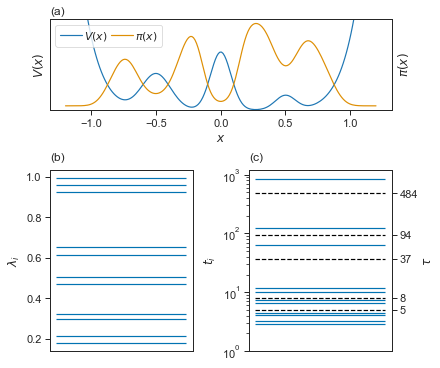
\includegraphics[width=0.8\textwidth]{chapters/hmm_selection/figures/prinz_pot.png}
    \label{fig:prinz}
\end{figure}

The Prinz potential \cite{prinzMarkovModelsMolecular2011} is shown in figure \ref{fig:prinz}.  Panel (a) shows the four well potential, $V(x)$, in blue and the stationary distribution, $\pi(x)$, showing the four metastable states, in orange. Panel (b) show the  ratio of successive eigenvalues resolvable by a  MSM with $\tau=5$. The large gap between the fourth and fifth eigenvalues (where $\lambda_1=1$) implies four metastable states. Panel (c) shows the exact ratio of implied timescales. The implied timescales show the largest gap between the second and third implied timescale. From this potential $100$ independent trajectories were sampled, initialized from random draws from the stationary distribution, discretised into 410 discrete states and used as data for estimating the HMMs in this work. See appendix \ref{app:hmm} for full details of the Prinz potential and simulation details. Panel (d) shows the mean implied timescales and \SI{95}{\percent} credible intervals as a function of the Markov lag time estimated with a Bayesian HMM, with the exact timescales shown as solid lines. The estimated timescales within statistical uncertainty for all values of $\tau$ except for $t_{4}$ for $\tau < 8$.  The number of hidden states was determined by the lag time and the exact timescales of the full Prinz transfer operator (see table \ref{tab:prinz_its_exact}). For example for $\tau = 130$ only $t_2 = 844$ is resolvable so a two hidden state HMM was used. The time and rate units used throughout this chapter are in terms of the time-step used to integrate the equations of motion, $\Delta t = 0.001$, and the distance units are arbitrary, see section \label{sec:app_hmm_prinz}.

\subsection{Model selection criteria}

In the following exposition, the likelihood, $L$ of the HMM parameters will feature heavily and so is repeated here for convenience \cite{noeProjectedHiddenMarkov2013a}: 

\begin{equation}\label{eqn:obs_lik_full}
\begin{split}
    L(\tilde{\mathbf{T}}, \mathbf{E}| \{s_t\}) & = \mathbb{P}(\{s_t\} | \tilde{\mathbf{T}}, \mathbf{E}) \\
    & = \sum_{\substack{\{h_t\} \in \\ \text{all paths}}} \tilde{\pi}_{h_{0}}E_{ h_{0}, s_{0}}\prod_{t=1}^{t_{max}}\tilde{T}_{h_{t-1}, h_t}E_{h_t, s_t}    
\end{split}
\end{equation}

This is the likelihood of the transition matrix and emission matrix ($\tilde{\mathbf{T}}, \mathbf{E}$ respectively) given the trajectory of observed states $\{s_t\}$. The multiplicand represents the probability of observing Markovian transition between hidden states (the $\tilde{T}_{h_{t-1}, h_{t}}$ term) and  observing the observed state (the $E_{h_t, s_t}$ term). The summand represents summing the probability over all possible combinations (paths) of hidden states ($\tilde{\pi}_{h_{0}}E_{ h_{0}, s_{0}}$ is the probability of the initial hidden state/observed state pair). This summation is infeasible for even small numbers of hidden states and trajectory lengths (e.g. for $2$ hidden states and a trajectory of $100$ frames, this is approximately $10^{30}$ potential paths). The Baum-Welch algorithm \cite{rabinerTutorialHiddenMarkov1989} was developed to maximize the likelihood through expectation maximisation. The details of this algorithm for maximum likelihood HMMs can be found in \cite{noeProjectedHiddenMarkov2013a}.  The maximum likelihood estimates of the parameters will be denoted $\hat{\theta}$, so the maximum of the likelihood function will be denoted $L(\hat{\theta}|\{s\})$. 

The optimal values of the CVLL and the AIC both minimize the \emph{Kullback-Leibler} divergence, $D_{KL}(p||q)$ \cite{mclachlanFiniteMixtureModels2000}. This is a measure of the difference between a given probability distribution, $p(s)$ and a reference distribution, $q(s)$: 

\begin{equation}\label{eqn:kl_div}
\begin{split}
    D_{KL}\left(p||q\right) & = \int q(s) \log{\left(\frac{ q(s) }{p(s)}  \right)} \mathrm{d}s \\ 
    & = \int q(s) \log{\left(q(s)\right)}\mathrm{d}s - \int q(s)\log{\left(p(s)\right)} \mathrm{d}s
\end{split}
\end{equation}

When the two distributions are the same $D_{KL} = 0$. The first term is the average information of, $q(s)$, also known as the information entropy \cite{mackay2003information}. The second term is average information of $p(s)$ but averaged over reference distribution. In the context of model selection, $p(s)$ is taken to be the modelled distribution $p(s|\hat{\theta})$ and $q(s)$ is the unknown true distribution. As only the latter term is dependent on the modelling choices and  $D_{KL}\ge 0$ (Jensen's inequality \cite{mackay2003information}) maximizing this term will lead to the model closest to the true distribution.  

The AIC approximates the second term in equation \ref{eqn:kl_div} and is defined as \cite{mclachlanFiniteMixtureModels2000}:
\begin{equation}\label{eqn:aic}
    \operatorname{AIC} = -2\log{\left(L\left(\hat{\theta}|\{s_t\}\right)\right)} + 2d
\end{equation}
where $d$ is the number of degrees of freedom of the model. For a reversible Markov model with $g$ states this is: $d = \sfrac{1}{2}g(g-1) + (g-1)$ \cite{trendelkamp-schroerEstimationUncertaintyReversible2015b}. For coarse-graining of MSMs with $n$ microstates, the emission distribution for each hidden state in a HMM assigns a probability to each observed states (so $n$ parameters) with the restriction that they sum to $1$, so there are $n-1$ degrees of freedom from the emission distribution \emph{per hidden state}. So the total  degrees of freedom for such a HMM is
\begin{equation}\label{eqn:hmm_dof}
    d = \sfrac{1}{2}g(g-1) + (g-1) + g(n-1). 
\end{equation}
The derivation of the AIC starts by approximating the true distribution $q(s)$ with the empirical distribution, giving rise to the $\log{L\left(\hat{\theta}|\{s_t\} \right)}$ term.  This will naturally over-fit to the data and the $d$ term attempts to account for this. $d$ is only equal to the degrees of freedom of the model under the assumption that the true model is under consideration in the model selection procedure \cite{ripley_1996}.  The factor of $-2$ is there to make an equivalence with Mallows $C_p$ \cite{friedman2001elements}. The selected model is the one which has the smallest AIC. 

Instead of bias correction with the degrees of freedom, $d$, cross-validation can be used  \cite{celeuxSelectingHiddenMarkov2008}. The CVLL is calculated in the following way (note, this is different from the procedure in \cite{celeuxSelectingHiddenMarkov2008}): 
\begin{enumerate}
    \item The observed trajectories are split into $N = 10$ training $\{s_t\}^{i}$ and test $\{s_t\}^{-i}$, $i = 1, ..., N$ sets using 50:50 shuffle-split, as described in chapter \ref{chap:msm} section \ref{sec:methods}. 
    \item For each $i$, fit a HMM using the training data $\{s_t\}^{i}$. \label{} 
    \item Calculate the log-likelihood of the parameters using the test data,  $\log{\left(L(\hat{\theta}^{i}|\{s_t\}^{-i})\right)}$, with the forward part of the Baum-Welch algorithm (algorithm \ref{alg:baum_welch}. 
    \item The CVLL is the average over the splits: 
    \begin{equation}
        \operatorname{CVLL} = \frac{1}{N}\sum_{i}^{N}\log{\left(L\left(\hat{\theta}^{i} \middle | \{s\}^{-i}\right)\right)}
    \end{equation}
\end{enumerate}
There are two points of failure in this procedure. First, the HMM may fail to converge on a given fold. Second, the `forward' part of the Baum-Welch algorithm may fail to give a finite estimate for the log-likelihood. If either of these failures occurred, the CVLL value for that number of hidden states was considered invalid.  In order to make the values of the CVLL comparable to the other criteria the CVLL was multiplied by: $2$ to account for the parameters being estimated on half of the data (and the log-likelihood scales linearly with the number of observations), and then $-2$ to account for the same factor in the definition of AIC, BIC and ICL. Thus the \emph{minimum} of the CVLL determines the selected model.

The BIC comes from consideration of the integrated observed likelihood, $p(\{s_t\})$ used in the definition of the Bayes factor: 
\begin{equation}\label{eqn:obs_lik_int}
        p(\{s_t\}) = \int p\left(\{s_{t}\}\middle |\theta \right)p(\theta) \mathrm{d}\theta
\end{equation}
Here $p(\theta)$ is the prior distribution over the HMM parameters for a given model specification. The integrated likelihood selects the model with the greatest evidence for the observed states, i.e. the model with the highest posterior probability, given the observed states, taking into account the increased flexibility of more complex models \cite{mackay2003information}\cite{kassBayesFactors1995}. The BIC is an approximation to the logarithm of equation \ref{eqn:obs_lik_int} and is given by:
\begin{equation}\label{eqn:bic}
    \operatorname{BIC} = -2\log{\left(L\left(\hat{\theta}\middle| \{s_t\}\right)\right)} + d\log{\left(N_{obs}\right)}
\end{equation}
where $d$ is the degrees of freedom and $N_{obs}$ is the number of observations.  The difference in BIC between two models, $BIC_{1}-BIC_{2}$ is an approximation to the log of the Bayes factor, the selected model is then the one with the smallest BIC.  The derivation proceeds by expanding the log of the integrand in equation \ref{eqn:obs_lik_int},  $\log{\left(p\left(\{s_{t}\}\middle |\theta \right)\right)}$ is a Taylor series about $\hat{\theta}$ up to second order. The regularity conditions alluded to in the introduction amount to the ability to safely ignore the higher order terms in this expansion.  

The derivation of the ICL follows an analogous path to the BIC but takes as its starting point the integrated complete data likelihood: 
\begin{equation}\label{eqn:class_lik_int}
    p\left(\{(s_t, h_t)\}\right) = \int p\left(\{(s_{t}, h_{t})\}\middle |\theta \right)p(\theta) \mathrm{d}\theta
\end{equation}
The integrated complete likelihood selects the model with the greatest evidence for the observed states \emph{and} the hidden states. As the hidden states are not observed they are taken to be the state with the largest probability given the observed state i.e. $\arg\max_{i}p(h=i|s=j)$, calculated using $\hat{\theta}$, and are denoted $\{\hat{h}_{t}\}$. The ICL is an approximation to $\log{(p(\{(s_t, \hat{h}_t)\})}$ and is given by: 
\begin{equation}\label{eqn:icl}
\begin{split}
        \operatorname{ICL} &= -2\log{\left(L\left(\hat{\theta}\middle|\{s_t\}\right)\right)} + d\log{\left(N_{obs}\right)} +2\mathrm{Ent.}     \\
        & = \operatorname{BIC} + 2\mathrm{Ent.}
\end{split}
\end{equation}

The term $\mathrm{Ent}$ is classification entropy given by: 
\begin{equation}
\begin{split}
     \mathrm{Ent} & = \sum_{t}^{t_{max}} -\sum_{j}^{g} M_{s_{t}, j}\log{\left(M_{s_{t}, j}\right)}  \\ 
     & =\sum_{t}^{t_{max}} H\left(s_{t}; \mathbf{M}\right)
\end{split}
\end{equation}
Here $\mathbf{M}$ is the membership matrix  with elements $M_{i,j}= p(h=j|s=i)$ and $H$ is the information entropy $H(s_{t};\mathbf{M}) = -\sum_j M_{s_t, j}\log{\left(M_{s_t, j}\right)}$, or just $H(t)$. This entropy quantifies the uncertainty with which the model assigns the given observed state to a hidden state. For example in a two hidden state system an observed state which belongs equally to either hidden state 1 or 2, then the entropy for that observation is $H = \log{(2)}$. 


\subsection{Criteria calculation details}\label{sec:hmm_details}
There are a number of practical details in calculating the information criteria which need to be addressed. 

The number of observations, $N_{obs}$, needed for the BIC and ICL, was calculated as: 
\begin{equation}
    N_{obs} = q\cdot\frac{(t_{max} - \tau)}{\Delta t}
\end{equation}
where $q$ is the number of trajectories, $t_{max}$ is the length of each trajectory, $\tau$ is the lag time and  $\Delta t$ is the trajectory time-step. The total number of frames is $N_{frames} = q\cdot t_{max}/\Delta t$

The classification entropy was calculated using the hidden state probabilities calculated in the final iteration of the forward-backward algorithm: 
\begin{enumerate}
    \item For each observed state in a trajectory, $s_t$, the conditional probability, $\gamma_{i}(t)=p\left(h_{t}=i \mid s_t, \theta\right)$, is calculated in the `update' part of the forward-backward algorithm. 
    \item The entropy was calculated at each frame of the trajectory,  $H(t)=-\sum_{i}\gamma_{i}(t)\log{\left(\gamma_{i}(t)\right)}$ and then summed over the $t_{max}$ frames of a trajectory and then over the $q$ trajectories: $\mathrm{Ent} = \sum^{q} \sum_{t}^{t_{max}} H(t)$.
    \item $\mathrm{Ent}$ was scaled by a factor of $N_{obs}/N_{frames}$ to account for the fact that an observation is a pair of states $(s_{t}, s_{t+\tau})$.
\end{enumerate}
A second method was available, which in principle should give the same answer but which diverged by up to a factor of three from the previous method. The entropy was calculated using the membership matrix, itself calculated from the emission matrix, $\mathbf{E}$, and the stationary distributions of the hidden $\tilde{\pi}$ and observed $\pi$ states: 
\begin{equation}
    M_{ji} = E_{ij}\frac{\tilde{\pi}_{i}}{\pi_{j}}
\end{equation}
where $i$ labels the $g$ hidden states and $j$ the $n$ observed states. The entropy was calculated using $\mathbf{M}$ as: 
\begin{equation}\label{eqn:ent_v2}
    \mathrm{Ent} = N_{obs}\sum^{n}_{j}\pi_{j}\sum^{g}_{i} M_{ji}\log{\left(M_{ji}\right)}
\end{equation}
The first method was deemed more accurate as the values of $\mathbf{M}$ contained potentially more numerical errors from equation \ref{eqn:ent_v2}. 

\subsection{Model selection}
The model selection criteria were used to select the optimum number of hidden states in a maximum likelihood HMM, using the discrete trajectories sampled from the Prinz potential. Five different values of the Markov lag time were used: $\tau=5, 8, 15, 65, 130$. These values were chosen because they resolve, respectively $7, 5, 3, 2, 1$ implied timescales in the full MSM state space, and as the top three of these timescales are dominant (see figure \ref{fig:prinz_pot} panel (b)), these values of $\tau$ resolve $4, 4, 4, 3, 2$ metastable states \cite{noeProjectedHiddenMarkov2013a} respectively. 

The data used to estimate the HMMs gave the exact relaxation timescales to within sampling error as shown  \ref{fig:prinz}, panel (d).  The implied timescales here were calculated by estimating HMMs using the true number of states for each value of $\tau$.  Also shown are the chosen values of $\tau$, they are denoted by vertical black lines. 

For each value of $\tau$ maximum likelihood HMMs were estimated with $g = 2 - 10$ hidden states. For each of the $45$ model specifications the model selection criteria were calculated  and the number of hidden states selected by each was compared to the true value. 

\section{Results and discussion}\label{sec:hmm_results}
\begin{table}
    \centering
    \mycaption{\textbf{Hidden state selection results.} The selected number of hidden states, $\hat{g}$, by the CVLL, AIC, BIC and ICL for each value of $\tau$. The true values, $g^{\mathrm{true}}$ are also shown. The asterisk highlights where $\hat{g}=g^{\mathrm{true}}$. The number in parentheses shows $\hat{g}-g^{\mathrm{true}}$. }
    \begin{tabular}{|c|c|c|c|c|c|}
    \hline
    $\tau$ & $g^{\mathrm{true}}$ & CVLL & AIC & BIC & ICL  \\
    \hline\hline
     $5$  & $4$ & $4^{*} (0)$  & $10 (6)$ & $10 (6)$ & $5 (1)$ \\
     $8$  & $4$ & $4^{*} (0)$ & $10 (6)$ & $8 (4)$  & $4^{*} (0)$  \\
     $15$ & $4$ & $4^{*} (0)$  & $9 (5)$ & $6 (2)$  & $4^{*} (0)$  \\
     $65 $& $3$ & $4 (1)$  & $5 (2)$  & $4 (1)$  & $3^{*} (0)$  \\
     $130$& $2$ & $4 (2)$  & $4 (2)$  & $3 (1)$  & $3 (1)$  \\
     \hline
    \end{tabular}
    \label{tab:prinz_criteria_results}
\end{table}

\begin{figure}
    \centering
    \mycaption{\textbf{Hidden state selection criteria}. Rows (a) - (e) show the selection criteria for HMMs with $\tau=5, 8, 15, 65, 130$. The best performing number of hidden states is indicated by an arrow. Column (i) shows the cross-validated log-likelihood ($\operatorname{CVLL}$). Column (ii) shows the AIC. The log-likelihood term is shown in blue and the degrees of freedom penalty ($2d$) is shown in orange. Column (iii) shows the BIC. The penalty term $d\cdot\log{N_{obs}}$ is shown in green.  Column (iv) shows ICL. The classification entropy penalty term $2\cdot \mathrm{Ent}$ is shown in red. Missing values indicate the failure of the HMM to converge. All values have been scaled so the minimum value in each panel is $1$.}
    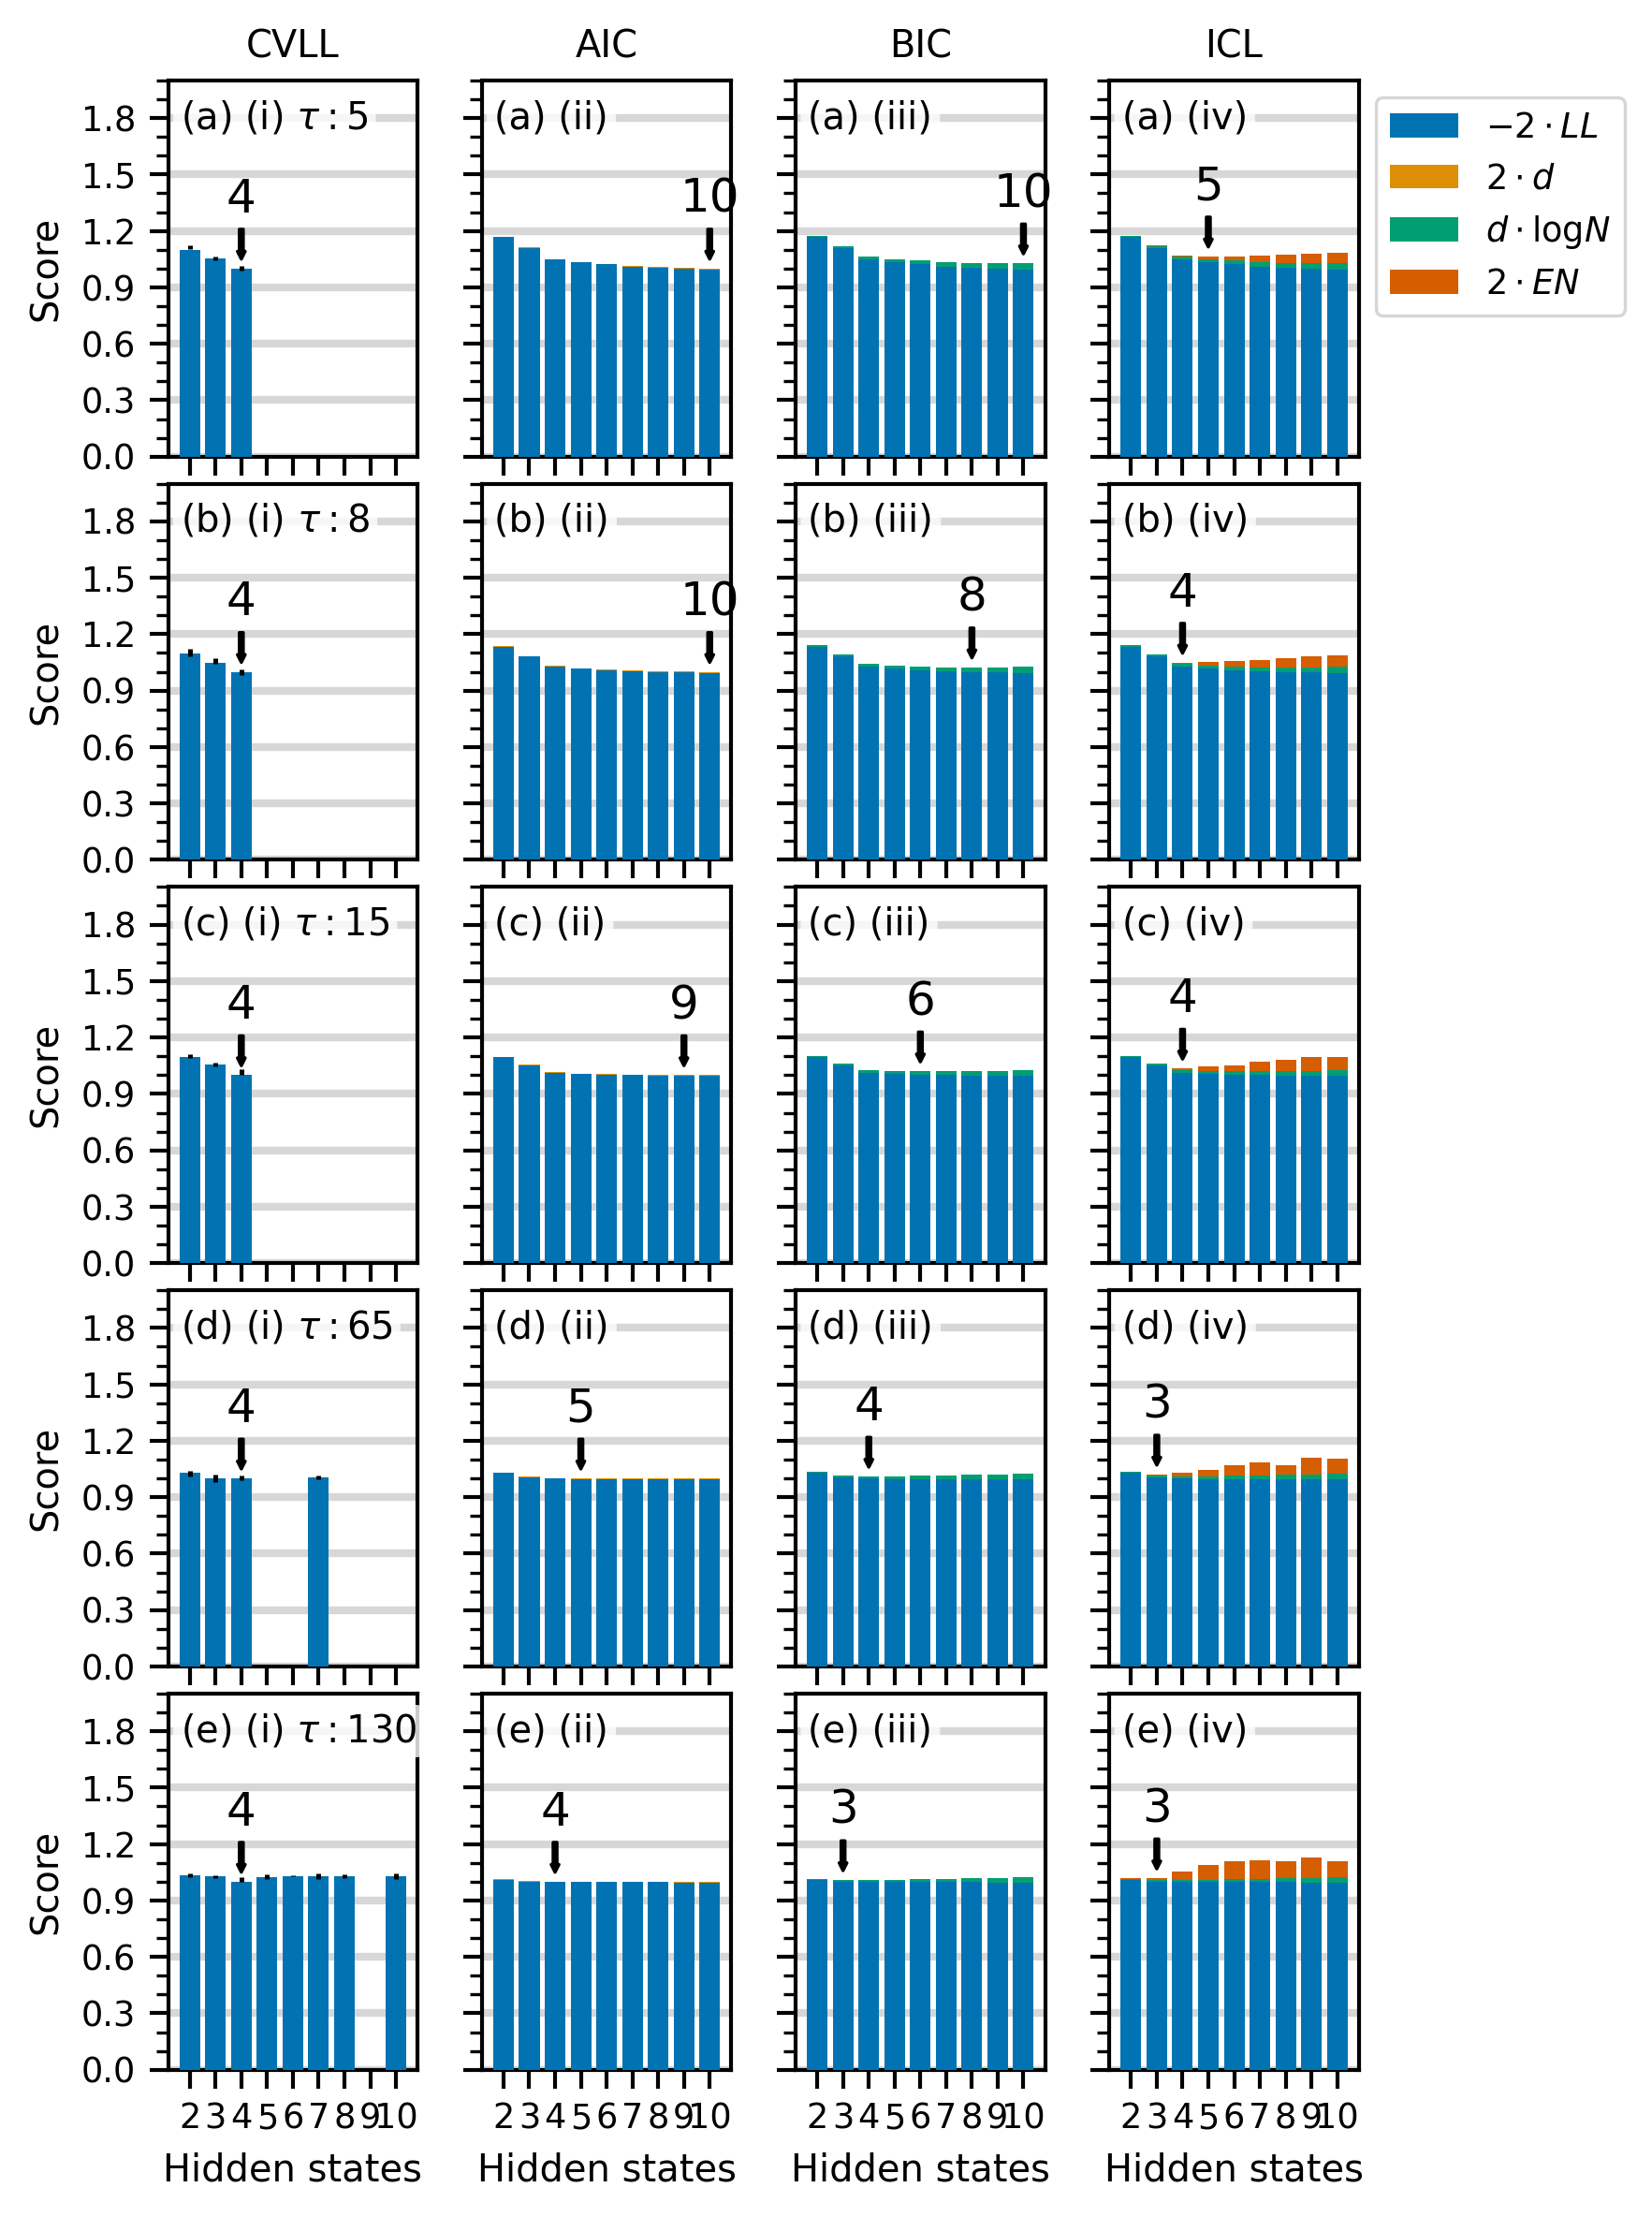
\includegraphics[width=0.75\textwidth]{chapters/hmm_selection/figures/prinz_h_state_selection.png}
    \label{fig:prinz_criteria_results}
\end{figure}

The selected number of hidden states using each criterion are shown in table \ref{tab:prinz_criteria_results}. The asterisk denotes when a criteria selects the number of hidden states equal to the number of metastable states. The relative values of the selection criteria are shown in figure \ref{fig:prinz_criteria_results}. Each row, (a) - (e), corresponds to a different value of the Markov lag time $\tau=5, 8, 15, 65, 130$. Each column, (i) - (iv), corresponds to the different model selection criteria, CVLL, AIC, BIC, and ICL. The minimum value of each criteria for each model is highlighted with an arrow indicating the selected number of hidden states, $\hat{g}$. The values are scaled so the value at the selected number of states is equal to $1$.  The coloured bars show the contributions of the different parts of each score. The blue bars shows the log-likelihood terms of equations \ref{eqn:aic}, \ref{eqn:bic} and \ref{eqn:icl} i.e.  $-2\times \log{\left(L(\hat{\theta}|\{s_t\})\right)}$. In the case of CVLL, the blue bars are the  cross-validated equivalent. The various penalty terms are shown in orange ($2d$ the AIC penalty), green ($d\log{N}$, the BIC penalty) and red ($2\mathrm{Ent.}$, the classification entropy). 

The ICL performs best by correctly identifying the number of hidden states for $\tau=8, 15, 65$. It fails at $\tau=5$ where the estimated implied timescales (figure \ref{fig:prinz}, panel (d)) show the dynamics of the hidden states are not quite Markovian. Although the selected value of $5$ is close to the true value of $4$, the ICL does not discriminate between $g=4 - 7$: their ICL values vary by less than \SI{1}{\percent}, as shown in figure \ref{fig:prinz_criteria_results} panel (a)(iv). It also fails at $\tau=130$, however the minimum value of the ICL is similar to the value for the true number of hidden states, $g = 2$, and is significantly different to the values for $g \ge 4$,  as shown in panel (e)(iv). In this case the ICL does distinguish between two  values of $g$ which include the true value on the one-hand, and the remaining values on the other. This behaviour is in contrast to the results in \cite{celeuxSelectingHiddenMarkov2008} in which the ICL correctly identified the number of hidden states for well separated emission distributions, and with large numbers of observations for less well separated distributions. However, for smaller numbers of observations with and less well separated clusters, the ICL under-estimated the number of hidden states. The ICL also under-estimates the number of clusters in the finite mixture context when the clusters are not well separated \cite{biernackiAssessingMixtureModel2000a}. 

The CVLL correctly selects four states for $\tau = 5, 8, 15$, however this was due failure of the cross-validation to produce a finite answer on some of the cross-validation folds. For example, for $\tau=5$, at least one cross-validation fold did not estimate the out-of-sample log-likelihood for $g\ge 4$. The remaining values are shown in figure \ref{fig:prinz_criteria_results} column (i). This causes problems with interpretation as is it is not clear whether failure is due to the  inefficiency of the cross-validation procedure or whether the given number of hidden states really has zero out-of-sample likelihood. The former is more likely given that models estimated on \SI{100}{\percent} of the data do converge and give interpretable answers. Given the lack of convergence for many of the values of $g$ comparison with the literature is difficult. The results in \cite{celeuxSelectingHiddenMarkov2008} show that the CVLL behaves similarly to the ICL but with less discrimination between values of $g$ i.e. in repeated experiments the distribution of selected values of $g$ was wider. In contrast, the results for $\tau=130$ in figure \ref{fig:prinz_criteria_results} panel (e)(i) show the CVLL over-estimates the number of hidden states.  Given the poor performance of the CVLL in this experiment it will not be discussed further here. 

The AIC overestimates for every value of $\tau$ and as $\tau$ increases the values of the AIC discriminate less between each value of $g$: for $\tau = 130$ the AIC for all $g$ are within \SI{2}{\percent} of each other. This is in contrast to the results in   \cite{celeuxSelectingHiddenMarkov2008} which the AIC selected the correct or underestimated the value of $g$. However, in simulation studies for finite mixtures (without the Markov regime) the AIC frequently over-estimated the number components \cite{celeuxEntropyCriterionAssessing1996}\cite{soromenho1994comparing}. The BIC also overestimates the number of hidden states for all values of $\tau$ but only by $1$ for $\tau=65, 130$. This is in contrast to the results in \cite{celeuxSelectingHiddenMarkov2008} for which the BIC behaved similarly to the ICL and either estimated correctly or under-estimated the number of hidden states.  For finite mixtures the BIC has been shown to under-estimates the numbers components \cite{biernackiAssessingMixtureModel2000a}. 

Although the AIC, BIC and ICL are derived from different starting points, they all take the form of the log-likelihood plus a penalty term, $b$:
\begin{equation}
    -2\log{\left(L\left(\hat{\theta}; \{s_t\}\right)\right)} + b
\end{equation}
The $b$ term in each case penalises the complexity of each model. The behaviour of these criteria can be understood in terms of the interplay between these two terms. The log-likelihood (the blue bars in columns (ii)-(iv) of figure \ref{fig:prinz_criteria_results}) monotonically increases with $g$ for all values of $\tau$. This is most pronounced for small values of $\tau$ (compare panel (a)(ii) to (e)(ii)), and demonstrates both over-fitting and the HMMs ability to capture the fast relaxation processes of the Prinz dynamics. Consider the $g=10$ model selected by the AIC for $\tau=8$, figure \ref{fig:prinz_tau8_g10} (the results are similar for $\tau=5$). This figure shows the sign structure of the exact relaxation processes (panels (a) - (c)) and those estimated from the HMM (panels (d) - (f)). The HMM captures the sign structure of the second and fifth relaxation process,  panels (d) and (e), as they have associated timescales larger than $\tau$, ($t_{2}=844.4, t_{5} = 11.9 > \tau=8$) and are thus resolvable. The 10th estimated relaxation process (panel (f)) is clearly spurious - the estimated timescale $\hat{t}_{10} = 4.0$ is less than the lag time, $\tau$, and the sign structure does not match that of the exact process, panel (c). For larger values of $\tau$ and $\tau= 130$ in particular (figure \ref{fig:prinz_criteria_results} panel (e)(ii)), the likelihood remains constant. This is because there is only one resolvable true relaxation process and increasing the number of hidden states just over-fits to spurious relaxation processes [REA: needs checking].  

\begin{figure}
    \centering
    \mycaption{\textbf{Comparison of estimated and true Prinz potential dynamics}. The true Prinz potential are compared with a HMM with $\tau=8$ and $g=10$ hidden states. Panels (a) - (c) shows the sign structure of the 2nd, 5th and 10th right eigenvector of the Prinz potential ($\mathrm{sgn}[\Psi(x)]$, shaded area). The Prinz potential ($V(x)$, blue solid line) is shown for reference. The exact timescales are labelled on the top right as $t_{2/5/10}$.  Panels (d) - (f) show the sign structure of the hidden state relaxation processes, projected onto the observed states. The eigenvectors projected onto the observed state basis, $q_{2/5/10}(x) = \sum_{i} E_{i, x} \cdot \tilde{\Psi}_2(i)$ , are shown as dotted lines, the summands are shown as coloured lines. The shaded areas are $\mathrm{sgn}[q_{2/5/10}(x)]$. The estimated timescales are labelled on the tope right as $\hat{t}_{2/5/10}$. }
    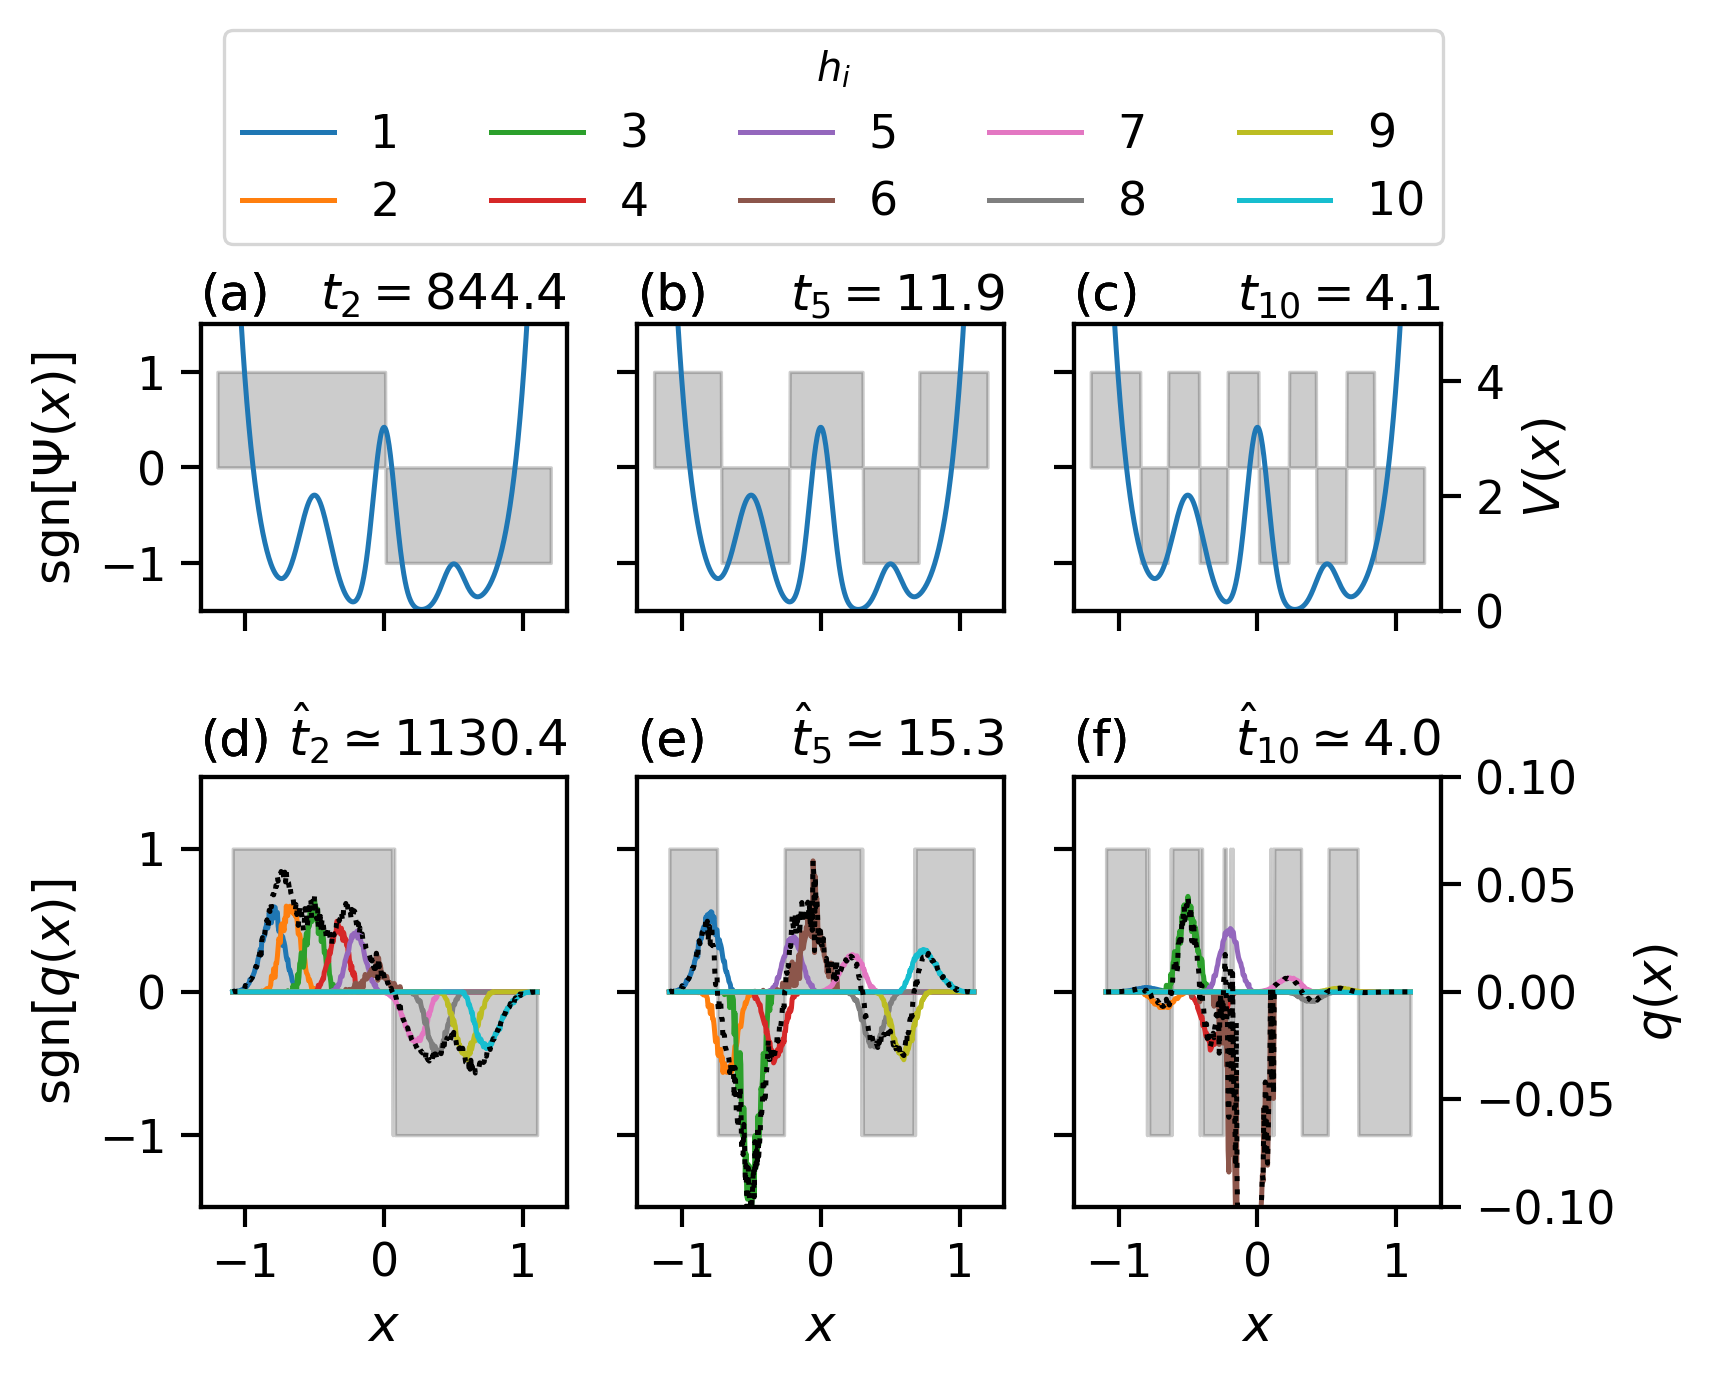
\includegraphics[width=0.8\textwidth]{chapters/hmm_selection/figures/hmm_tau_8_g_10.png}
    \label{fig:prinz_tau8_g10}
\end{figure}

The AIC the penalty term, $b=2d$ (orange bars in figure \ref{fig:prinz_criteria_results}, column (ii)), is there to correct the approximation of the KL divergence by log-likelihood. It increases proportional to $g^{2}$ but only affects the selected $g$ for $\tau=15, 65, 130$ (figure \ref{fig:prinz_criteria_results} panels (c), (d) and (e)(ii)). The origin of the BIC penalty term, $b=d\log{N_{obs}}$ (green bars, column (iii)) is to correct the approximation of the integrated likelihood by the maximum log-likelihood. The BIC over-estimates the number of hidden states albeit by a smaller number than the AIC, due to the penalty term rising faster with $g$ by a factor $\log{N_{obs}}/2$. 

\begin{figure}
    \centering
    \mycaption{\textbf{The classification entropy of HMMs}. Panels (a)-(c) show the emission distributions of HMMs with $\tau=8$ and $g = 2, 4, 10$ respectively. Each coloured line represents the emission distribution, $E_{i, x}$,  of the hidden states, $i$. Panels (d) - (f) show the information entropy for observed state at $x$, weighted by the stationary distribution over the observed states: $\pi(x)H(x)$. The label shows the average entropy per observation $Ent/N_{obs} = \sum_{x}\pi(x)H(x)$.}
    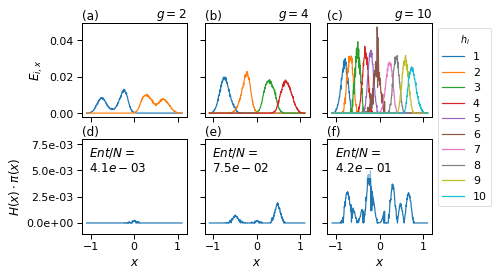
\includegraphics[width=0.8\textwidth]{chapters/hmm_selection/figures/prinz_entropy.png}
    \label{fig:prinz_ent}
\end{figure}

The ICL penalty term $b=d\log{N}+2\mathrm{Ent}$ corrects the approximation to the integrated complete data likelihood by the log-likelihood. It is comprised of the BIC penalty term (green bars in figure \ref{fig:prinz_criteria_results}) and the entropy term (red bars). This is associated with increasing $g$ directly through the BIC penalty term, $\simeq g^{2}\log{N_{obs}}$,  and indirectly due the overlap of emission distributions. This is demonstrated in figure \ref{fig:prinz_ent}. Panel (a) shows the emission distribution for a two state HMM. These two distributions only overlap around the high barrier at $x=0$. Panel (d) shows the entropy at each value of $x$, weighted by the stationary distribution over the observed states, $\pi(x)$. The information entropy is zero almost everywhere as each observed state can be assigned unambiguously to a hidden state. The exception is around $x=0$ where the entropy reaches its highest possible value of $\log{2}$. However, the average classification entropy per observation, $\sum_{x}\pi(x)H(x)$ is low as the fraction of observations at $x=0$, $\pi(0)$ is negligible. As the number of hidden states increases, panels (b) and (c), the  entropy increases because the emission distributions overlap more, and the average entropy increases because they overlap in regions which are visited more often i.e. where $\pi(x)$ has significant density (panels (e) and (f)). As column (iv) of figure \ref{fig:prinz_criteria_results} shows, the entropy penalty is the source of the success of the ICL in selecting  the correct number of hidden states. 

Minimizing the entropy penalty alone is similar to maximizing the crispness/scaling condition  in robust PCCA (equation 4.19 in \cite{deuflhardRobustPerronCluster2005b}) in that it maximizes the number of  observed states that are unambiguously assigned to one hidden state. However, the minimum entropy solution (ignoring the other terms) will always favour two hidden states separated by the slowest relaxation process, which for small $\tau$ doesn't capture the potential other metastable states. The ICL balances the need for a `crisp' assignment with the need for hidden states needed to accurately  model the transition matrix. 
\section{Conclusions}\label{sec:hmm_conclusions}
Four model selection criteria have been compared for identifying the number of hidden states in HMMs of dynamics simulated from the four-well Prinz potential. The four criteria fall into two categories - those than aim to minimize the Kullback-Liebler divergence, the CVLL and the AIC, and the those that maximize an integrated likelihood, the BIC and ICL. The CVLL was of limited usefulness because it was unable to produce results for a significant proportion of the models tested and because of its relatively large computational requirement. The AIC and BIC both overestimated the number of hidden states although the BIC by fewer states than the AIC. These results do not match the results from previous studies on selecting the number of components in mixture models and in HMMs. The ICL, which maximizes the integrated complete data likelihood performed best by correctly identifying three out of five hidden states and where it failed it only overestimated one extra hidden state. 

The integrated completed data likelihood is a natural criterion for the purpose of coarse graining  MSMs of conformational dynamics. The penalisation term in the ICL is aligned with assumptions that make metastable Markov processes amenable to coarse graining with a HMM. The purpose of coarse graining is to provide an interpretable model of dynamics which means balancing simplicity and accuracy. Part of the simplicity of a coarse grained model is being able to interpret given structures (microstates) as belonging to a particular metastable state. Considering the integrated classification likelihood naturally penalises less interpretable solutions by considering the models' evidence for both the observed states and the classification into hidden states. 

However, the ICL did not perform perfectly and testing this criteria on a single test case does not prove its general usefulness. Further work is needed to justify its routine use. First further benchmark systems are needed to test whether it identifies  metastable states in well-known systems, e.g., alanine dipeptide. Second, the failure of the BIC in this case is unexpected and it should be possible to calibrate both the ICL and the BIC against the `exact' values of integrated observed, and classification likelihood, using MCMC. This would help to establish whether the source of the failure of both criteria was the assumptions behind their derivation or from the task of coarse graining approximations of metastable Markov processes. 
